% !TEX root = ../main.tex

% 报告主体

%%%
%---------------------------------------------------------------------
% 实验
\clearpage
\JMSection{实验过程}
\subsection{实验前期准备}

\subsubsection{接线准备}

由于实验台的选择,本小组主要完成对于超导转变温度的测量,这里就需要对于样品的电阻进行测量,对于测量电路的接线,主要通过如下所示的接线图来进行:
\begin{figure}[{H}]
	\centering
	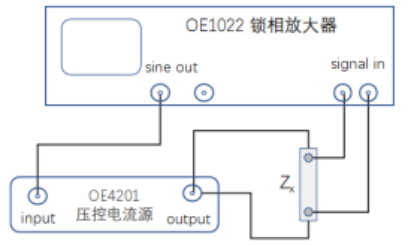
\includegraphics[width=0.45\linewidth]{pre3.png}
	\caption{交流四引线法}
	\label{}
\end{figure}

实际操作过程中,对于实验线路操作,经过了很多尝试,由于对于接线过程中相关器件的内部结构的不熟悉,经历了很多次纠错的经过,最终接线如下:
\begin{figure}[{H}]
	\centering
	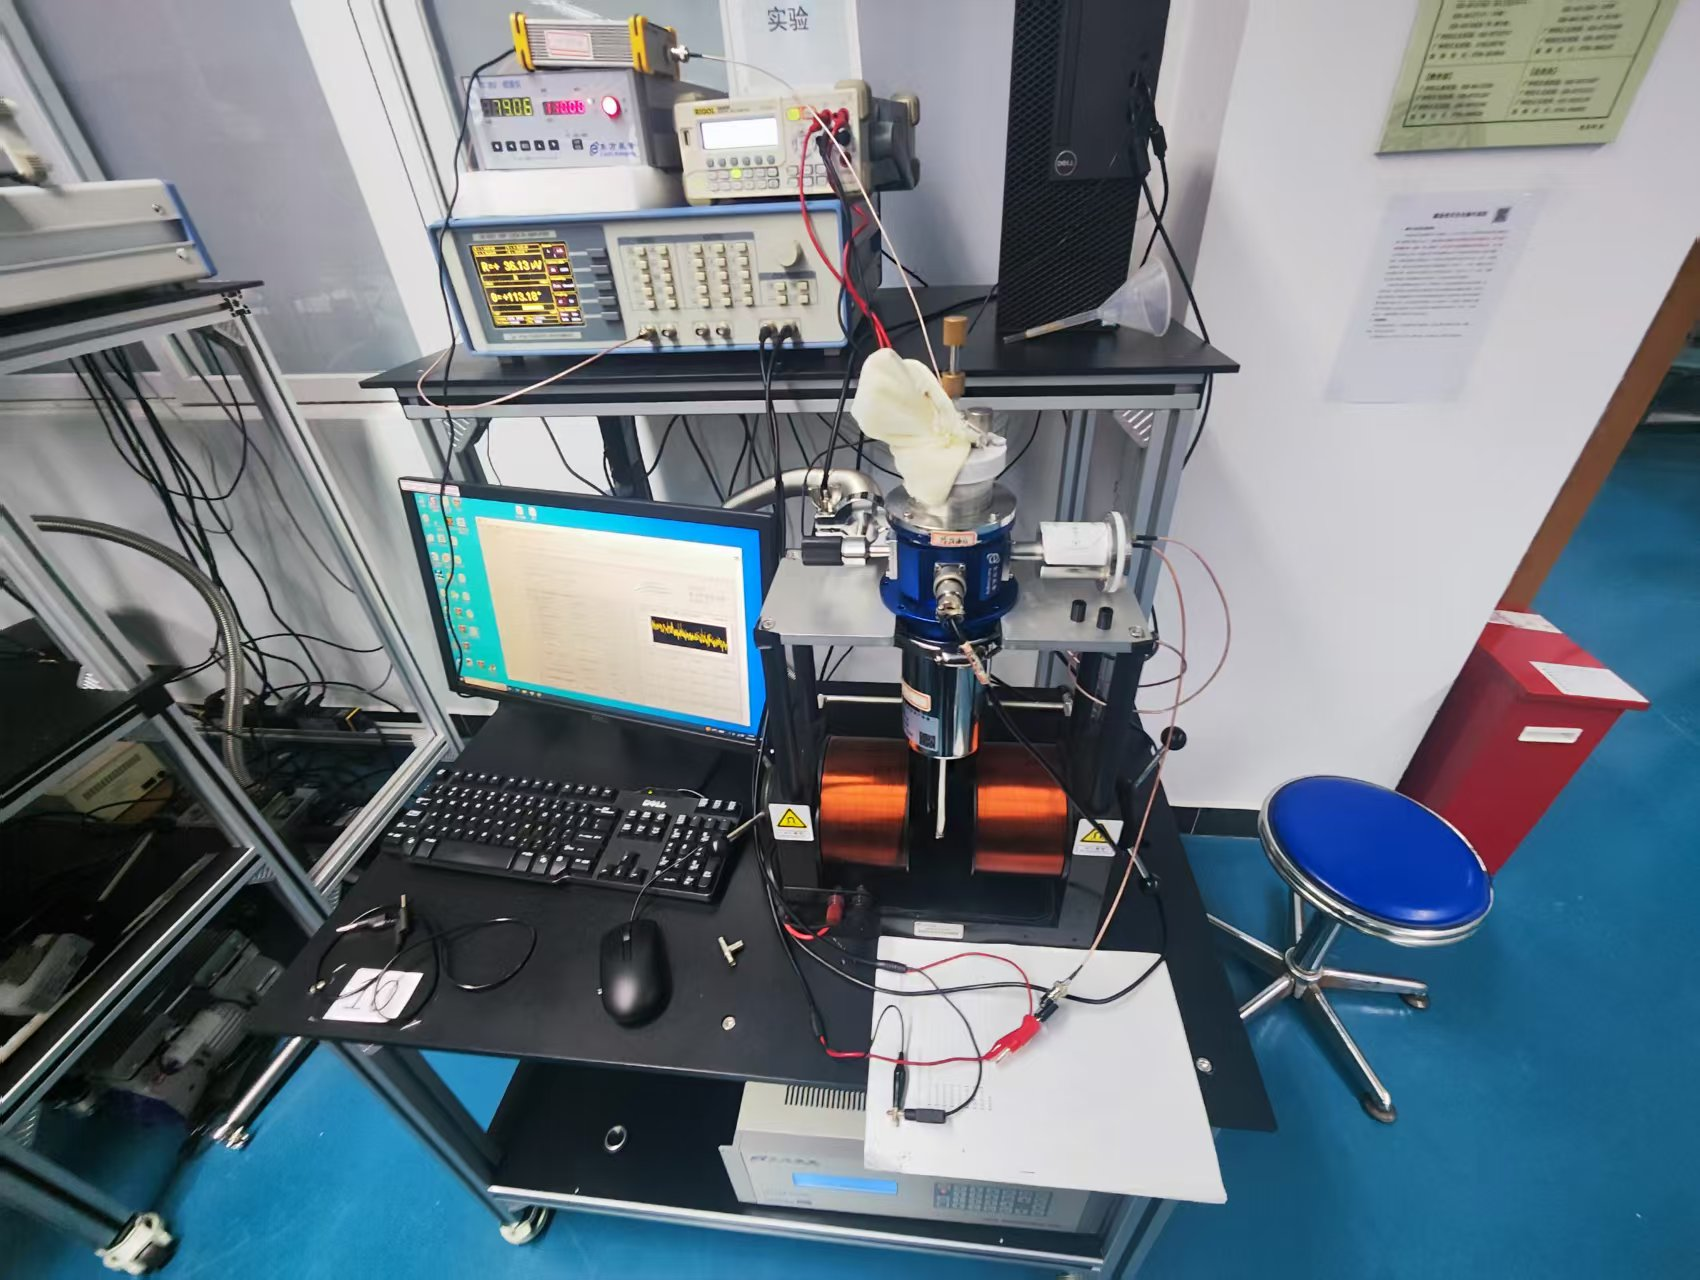
\includegraphics[width=0.7\linewidth]{body1.jpg}
	\caption{实际接线图}
	\label{}
\end{figure}

\subsubsection{温度准备}

实验主要通过液氮降温,对于理论的转变温度来说,液氮理论上已经满足实验所需的温度条件,\JMEmph{但是实际操作过程中,我们发现,实际上根据Pt1000给出的数值再与讲义后的对照表进行对照,发现温度与控温器给出的温度相差很大,这一点会在分析讨论部分给出本小组的意见。}

除了常规液氮降温,在实验过程中,\JMEmph{在老师的启发下,本小组将恒温器液氮部分的出气口连接到一个抽气泵,通过加快液氮蒸发的速度,从而达到更低温度的效果,但是实际实验结果来看,效果并没有达到预期。}

\subsubsection{LabVIEW准备}

实验软件的准备也同样出现了很多问题,基本上也属于摸索阶段,对于接口的试错导致不得不一次又一次进行重启软件,最后得出了如下接口对应关系:

\begin{itemize}
	\item \textbf{控温仪 TC202}  $\rightarrow$ COM7
	\item \textbf{3058E} $\rightarrow$ USB0::0X1
	\item \textbf{电磁铁电源} $\rightarrow$ COM1
	\item \textbf{锁相放大器} $\rightarrow$ COM3
\end{itemize}



\subsection{转变温度测量}
温度区间取80k至110k(绘图时对于数据进行了裁剪),功率采用15\%,升温降温分别测量,最终得出的实验数据绘图后显示为:
\begin{figure}[{H}]
	\centering
	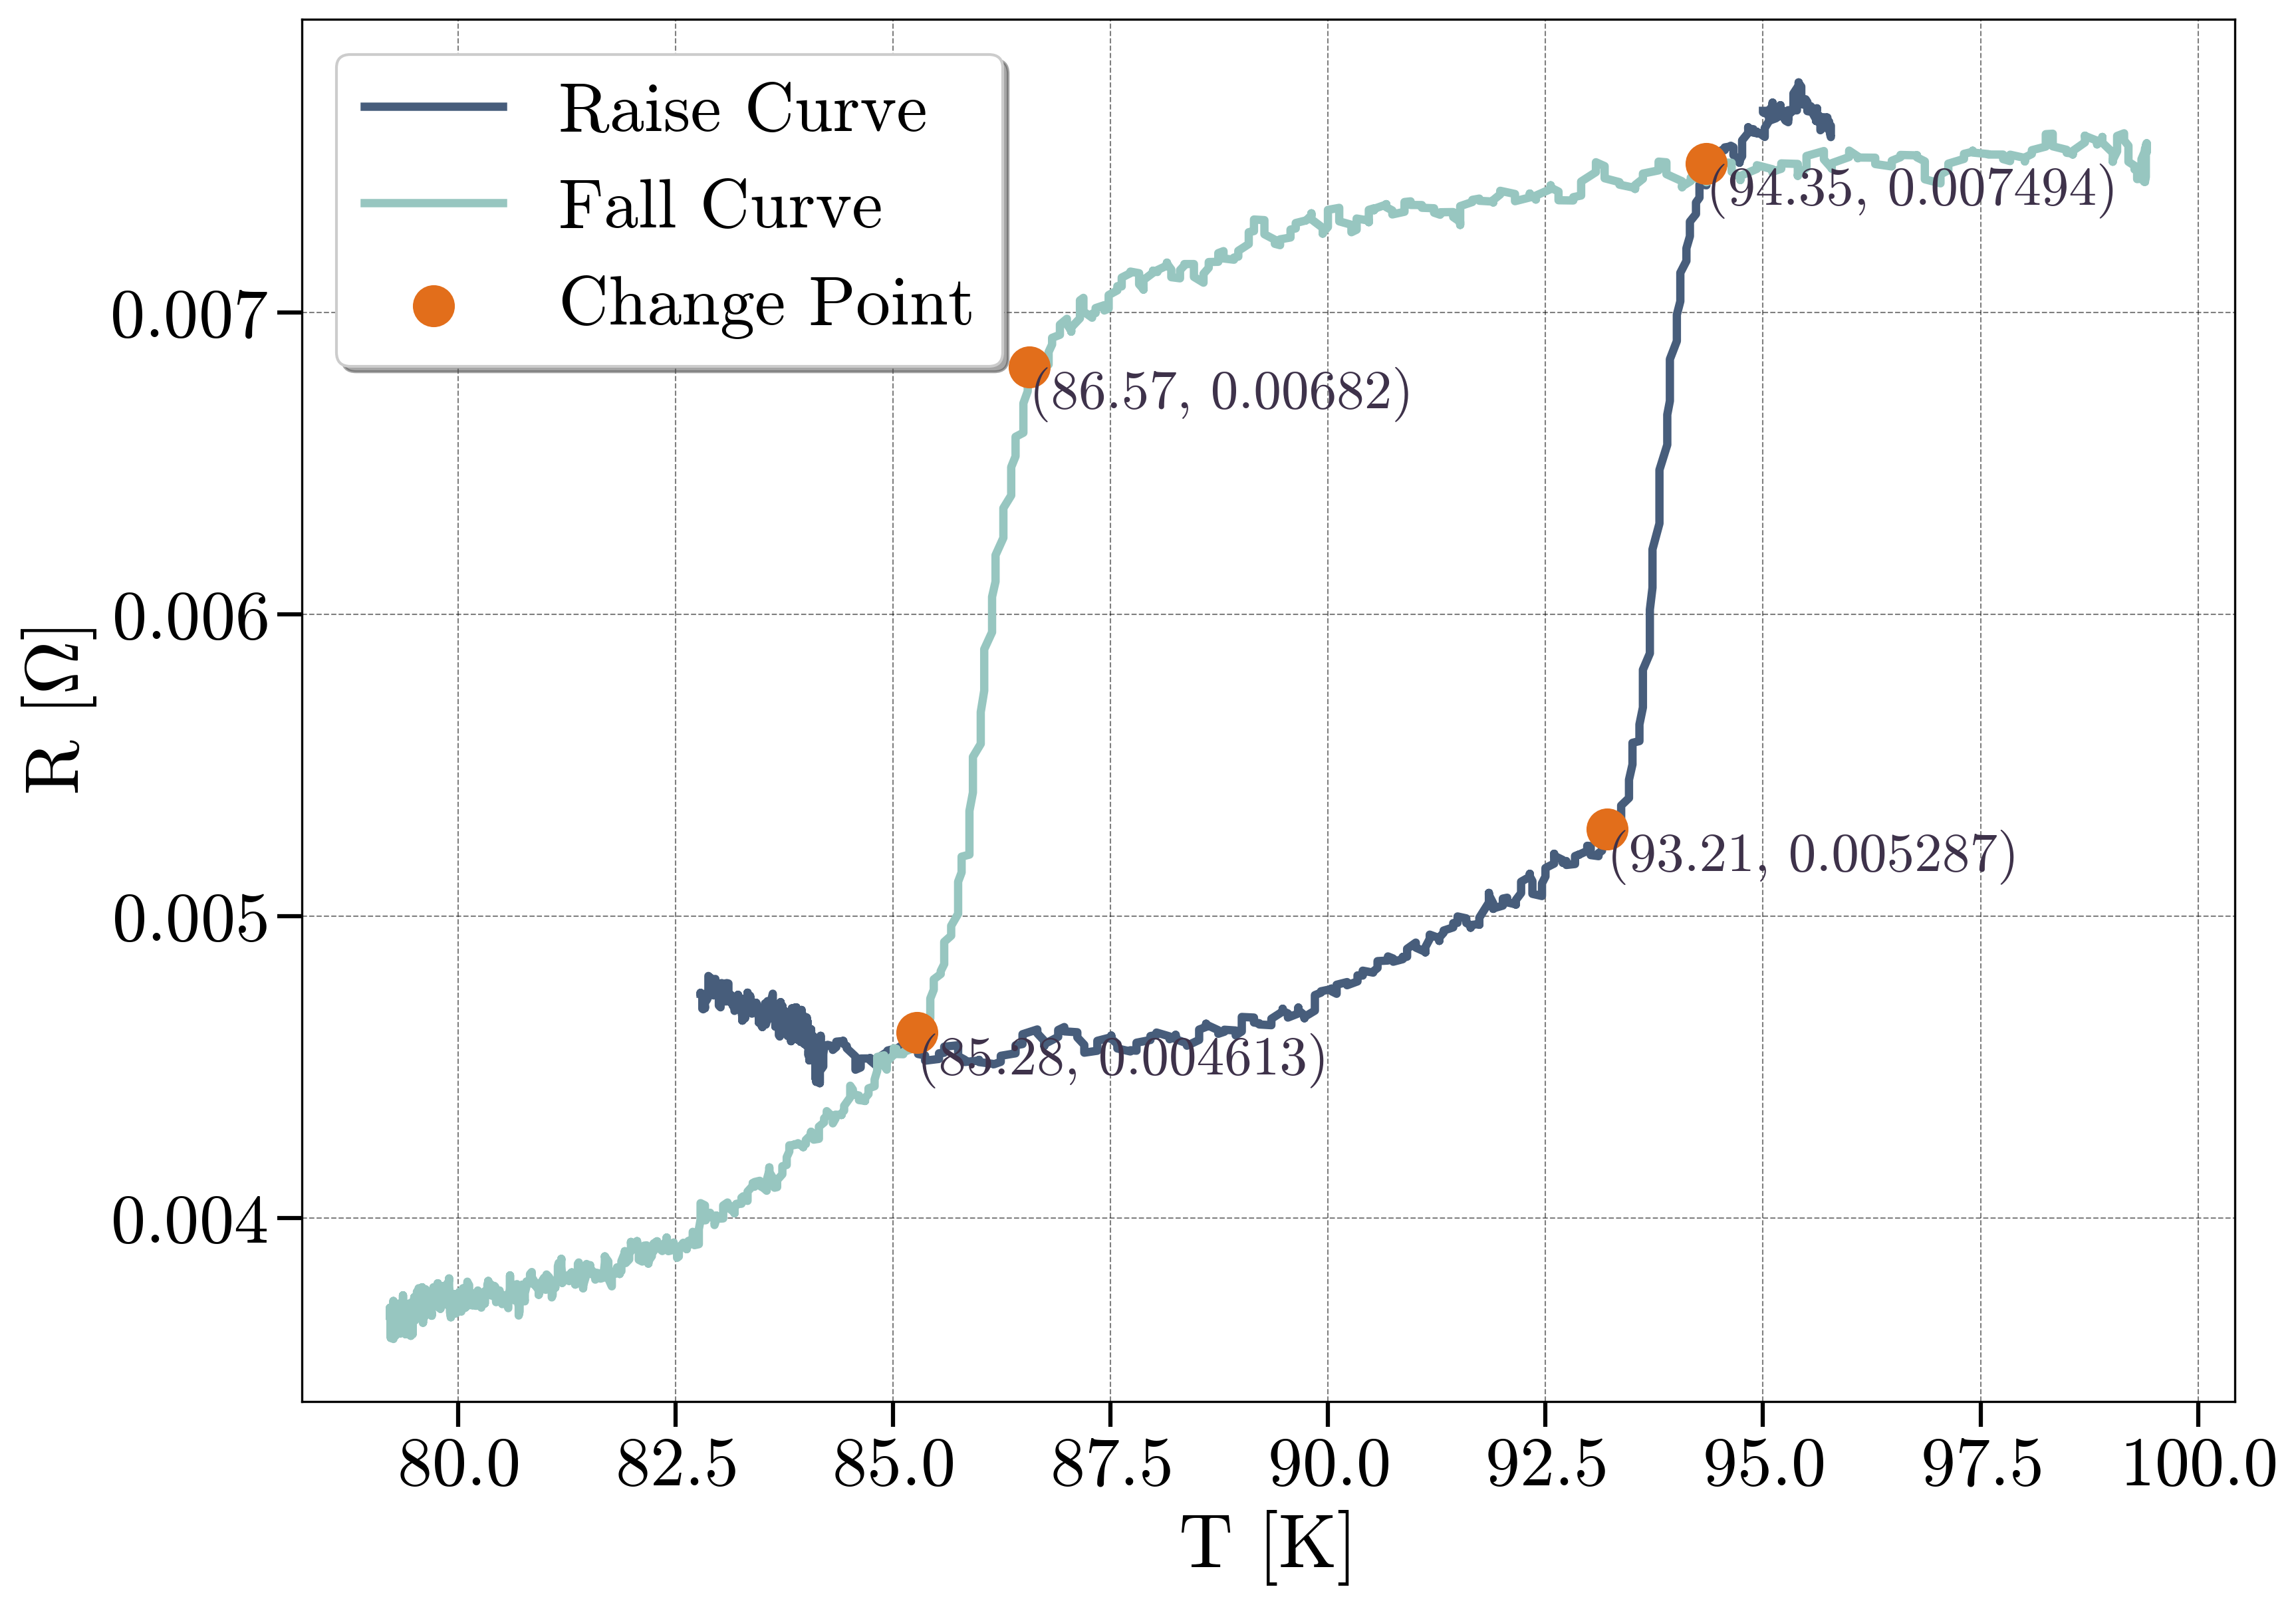
\includegraphics[width=0.7\linewidth]{body2.png}
	\caption{升温与降温转变温度}
	\label{}
\end{figure}

\subsection{外加磁场对样品转变温度影响}
\subsubsection{实验过程}
本实验是选择了讲义中给出的众多实验问题中其中一个:

\highlight{外磁场或外加电流如何影响超导转变时的电阻随温度($T_c$)的变化?}

\JMEmph{相关实验方案已经在本实验报告预习报告部分给出了,本方案于实验的第二周进行。}

其中与讲义不同的是,讲义中给出需采用电磁铁电源中的磁场模式(FIELD),但是在本实验中采用的是电流模式,故通过特斯拉计测量出如下电流与磁场对应关系:

\begin{table}[h!]
	\centering
	\renewcommand{\arraystretch}{1.5} % 调整行高
	\caption{电流与磁场的关系}
	\label{tab:current_magnetic_field}
	\begin{tabular}{|c|c|c|c|c|c|c|c|c|}
		\hline
		\textbf{电流/A} & 1 & 2 & 3 & 4 & 5 & 6 & 7 & 8\\ \hline
		\textbf{磁场/KGS} & 0.6732 & 1.2414 & 1.8436 & 2.4955 & 3.0319 & 3.6071 & 4.1647 & 4.7109\\ \hline
	\end{tabular}
\end{table}


最终数据输出结果如下,相关数据讨论见分析讨论部分:
\begin{figure}[{H}]
	\centering
	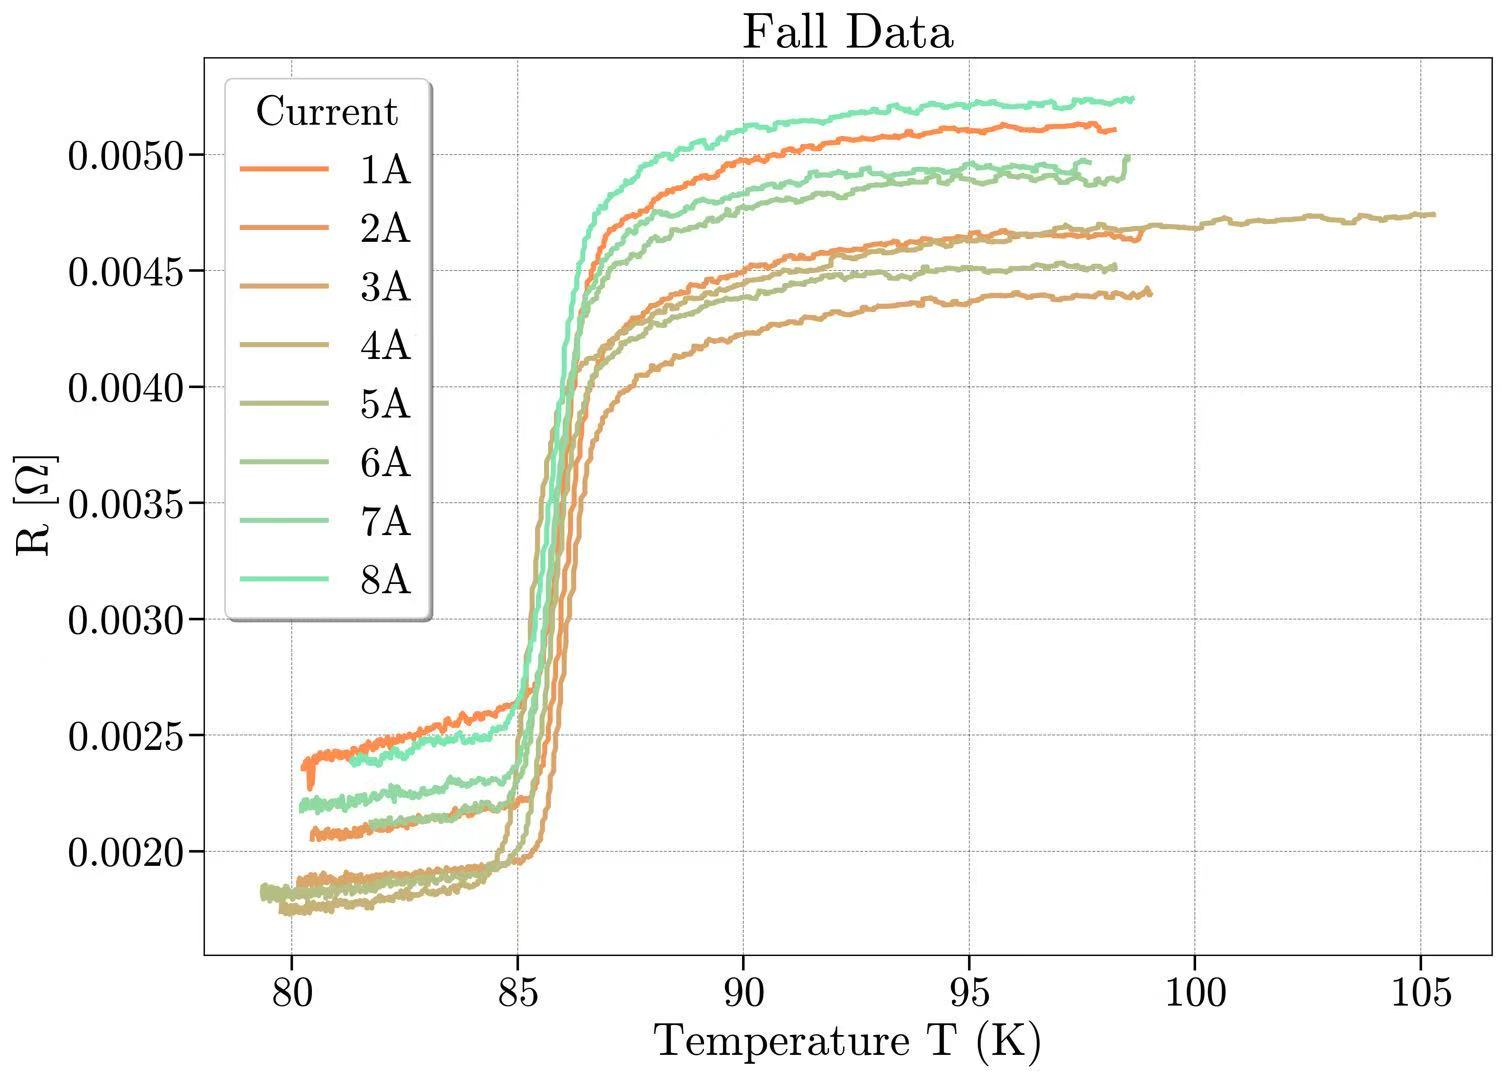
\includegraphics[width=0.8\linewidth]{body3.jpg}
	\caption{不同线圈电流下,样品在降温过程的电阻变化}
	\label{11}
\end{figure}
\begin{figure}[{H}]
	\centering
	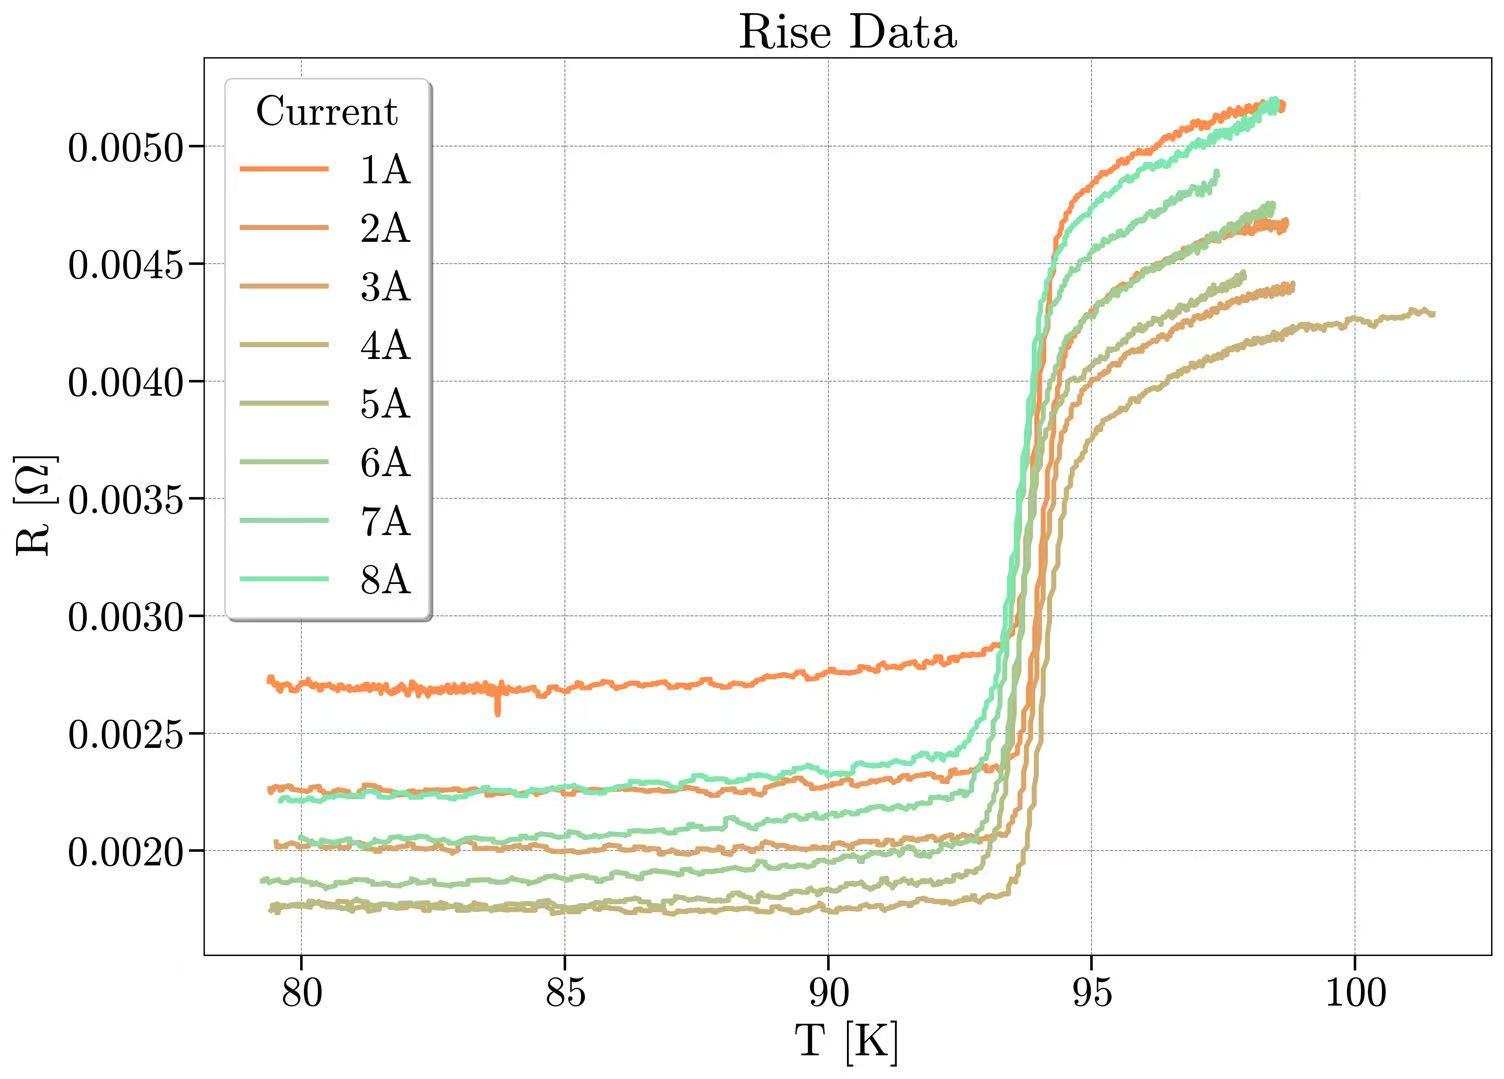
\includegraphics[width=0.8\linewidth]{body4.jpg}
	\caption{不同线圈电流下,样品在升温过程的电阻变化}
	\label{22}
\end{figure}


\subsubsection{初步讨论}

从实验结果来看,并不能一个能够分析出规律的结果。

在实验现场当我们发现这个问题后,经过与老师讨论,通过的如下一系列操作优化实验:
\begin{itemize}
	\item 减小升温功率,之前为保证升温功率能够使得恒温器能够达到目标温度,采用了15\%挡位,但是考虑到可能会导致升温速率过快,器件传导不及时等问题,降低了升温功率为1\%,但是随之而来的问题就变为,当温度在84K左右时,已经无法升温了,不得不再次调回15\%挡位,实际结果并没有区别。
	\item 调整液氮挡位,由于考虑到,液氮在器件中可能冷却能力不足,通过调整器件挡杆来调整液氮,但是实际上也收效甚微。
	\item 选择读取Pt1000给出的电阻值来进行温度换算,但是与实际温度对照表进行对照后,发现,大相径庭,如果选择Pt1000的数据作为实际测量温度的话,那么超导转变温度已经与实际测量温度相差甚远。
\end{itemize}

\JMEmph{尝试了众多优化方案后,依旧无法得出一个具有规律的实验结果,最终本小组决定采用最开始的实验数据进行分析,尽管没有完成实验预期,但是在分析讨论部分,我会给出个人对于实验优化方向的理解与讨论。}



\clearpage

%---------------------------------------------------------------------
% 分析与讨论
\JMSection{分析与讨论}

\subsection{数据分析}

\subsubsection{超导讨论}
对于判断待测样品是否为超导体,通常需要基于超导体的两个基本特性来进行判断。
这两个基本特性是:

\begin{enumerate}
    \item \textbf{零电阻性}:超导体在其临界温度以下会表现出零电阻性。当样品温度降到其超导转变温度(通常称为临界温度,$T_c$)以下时,其电阻将突然降为零,并且在整个超导状态下维持零电阻。通过测量电阻与温度的关系,可以确认这一点。如果在某一温度点电阻骤降至零,并在后续保持不变,则样品有可能是超导体。
    
    \item \textbf{完全抗磁性(迈斯纳效应)}:超导体具有完全抗磁性,也就是说,当超导体进入超导状态时,它会排斥磁场,表现为磁通量完全被排除在其内部。这种现象称为迈斯纳效应。实验上,通常通过测量样品在低于临界温度时的磁响应来确认这一点。如果在低于临界温度时样品的磁场强度显著减弱或消失,则说明样品可能具有迈斯纳效应,表明它可能是超导体。
\end{enumerate}

因此,要判断待测样品是否超导,实验中需要:
\begin{itemize}
    \item \textbf{测量电阻}:观察样品的电阻随温度变化的情况,确认是否存在零电阻的转变。
    \item \textbf{测量磁性}:使用磁场探测设备测量样品在临界温度以下的磁场响应,确认是否存在迈斯纳效应。
\end{itemize}

\subsubsection{超导转变温度}
\begin{figure}[H]
	\centering
	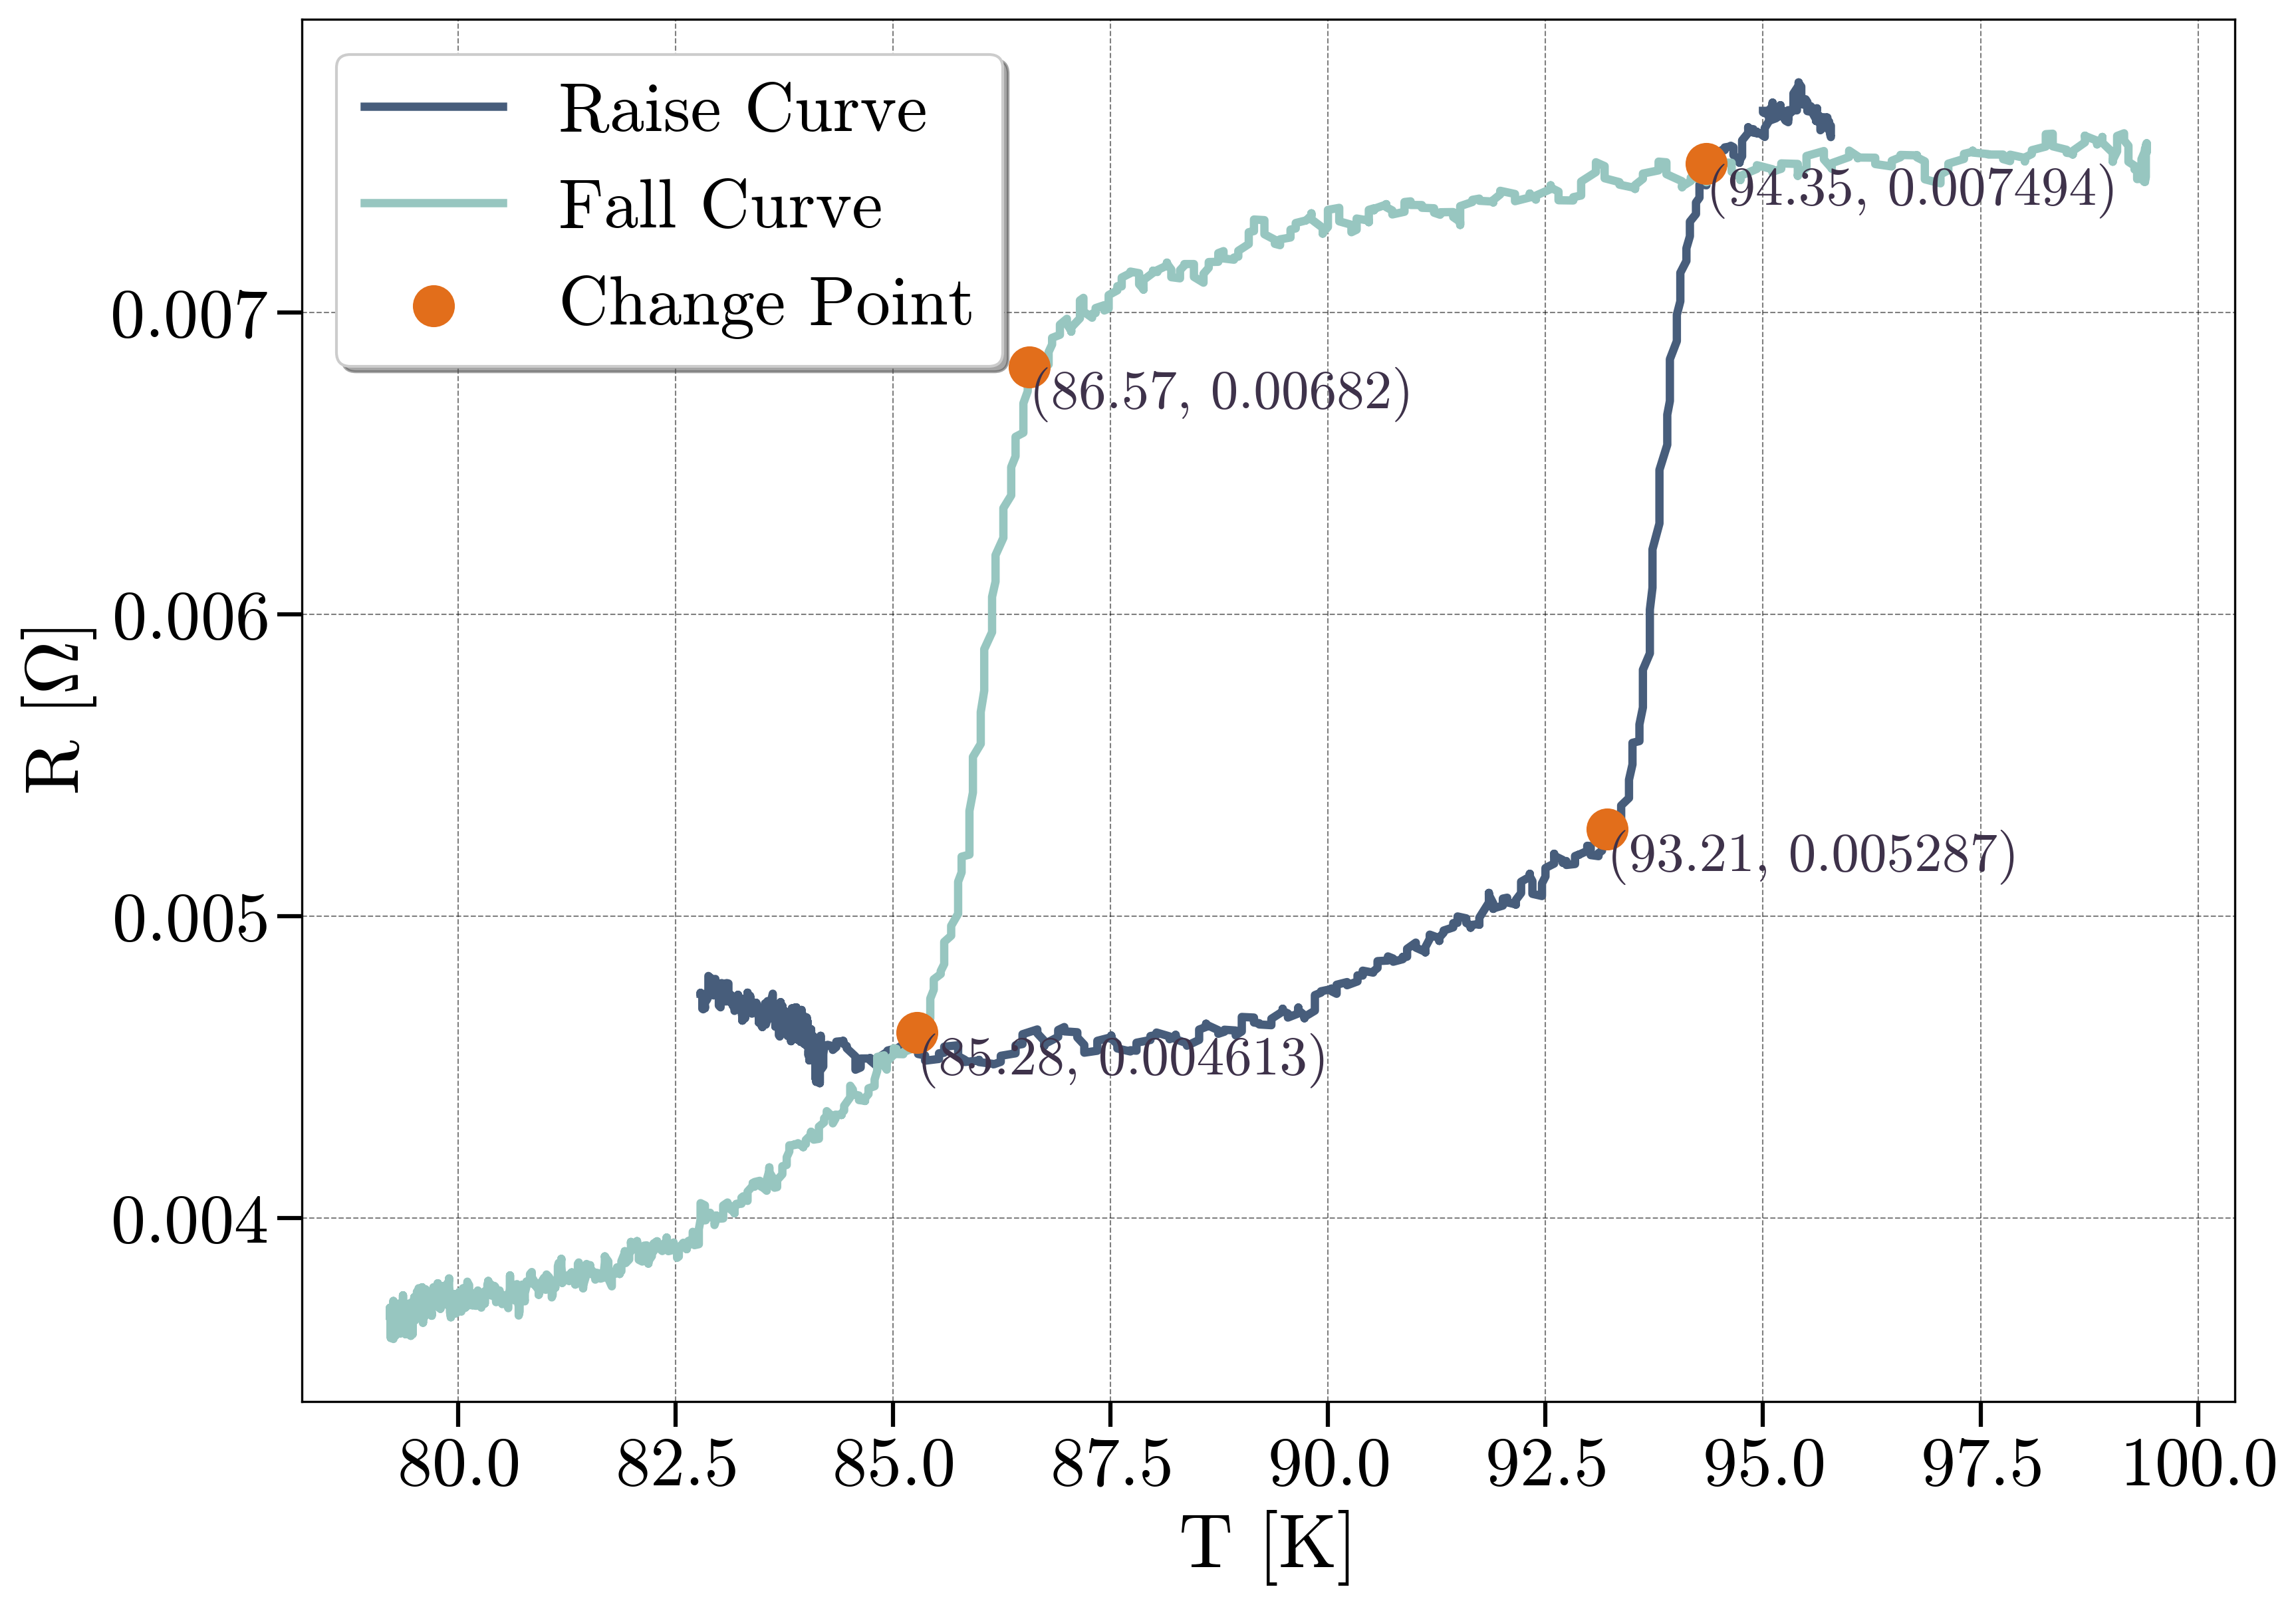
\includegraphics[width=0.7\linewidth]{day1.png}
	\caption{升温与降温转变温度}
	\label{fig:day1}
\end{figure}

第一周实验中,我们的重点是熟悉仪器,同时测量了一组数据,即“样本在温度升高和降低的条件下的电阻值”。数据绘制的图像如上图所示。

可以发现,\JMEmph{在升温过程中,温度在93.21K时,电阻值发生明显的转变,在94.35K时,电阻值转变开始趋于平缓;在降温过程中,温度在86.57K时,电阻值发生明显转变,在85.28K时,电阻值转变开始趋于平缓。}

上面的实验数据说明,该样品在\highlight{85K-94K存在超导转变现象。}

值得注意的是,升温过程的转变温度与降温过程的转变温度相差有\highlight{8K},显然在温度的测量中应该存在误差,这在后面再进行更详细的讨论。

\subsubsection{磁场对于超导转变温度影响}

在第二周的实验中,我们探究了被测样品在不同大小的外加磁场对样品转变温度的影响。实验数据的绘制图像如下所示:



我们将电阻值转变的部分截取出来,并标记出电阻值开始明显变化的点,如下所示。

\begin{figure}[H]
	\centering
	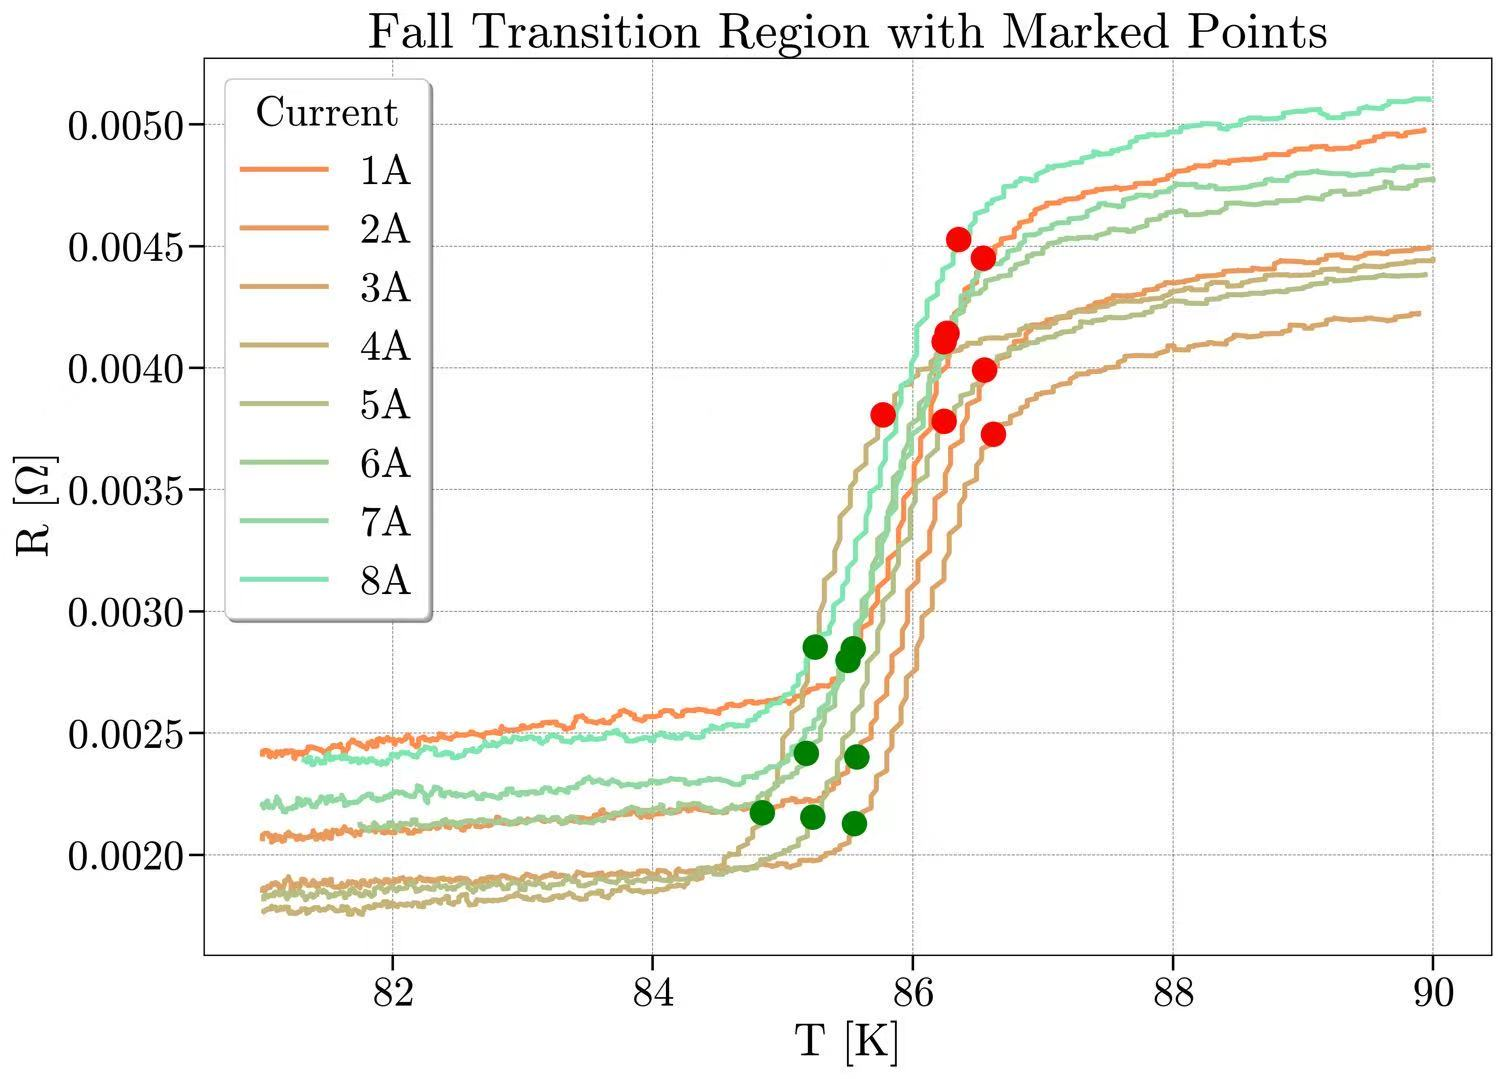
\includegraphics[width=0.7\linewidth]{1.jpg}
	\caption{电阻值转变开始变化的点}
	\label{fig:1}
\end{figure}

\begin{figure}[H]
	\centering
	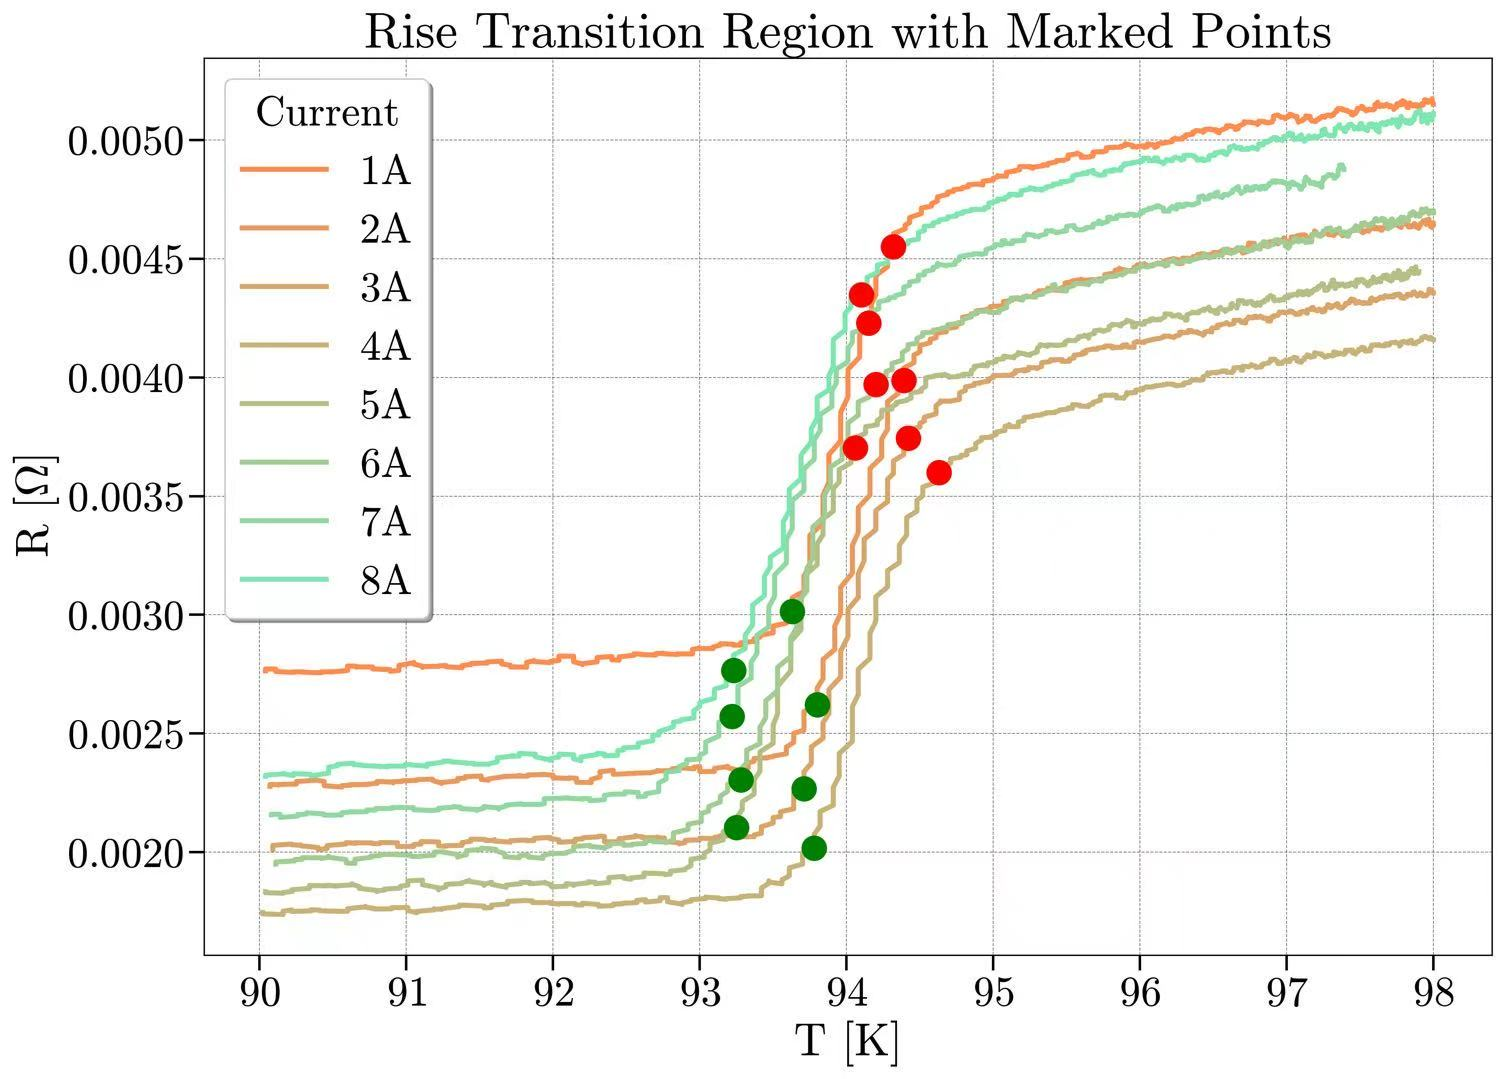
\includegraphics[width=0.7\linewidth]{2.jpg}
	\caption{电阻值转变开始变化的点}
	\label{fig:2}
\end{figure}

\begin{figure}[H]
	\centering
	\begin{minipage}{0.4\linewidth}
		\centering
		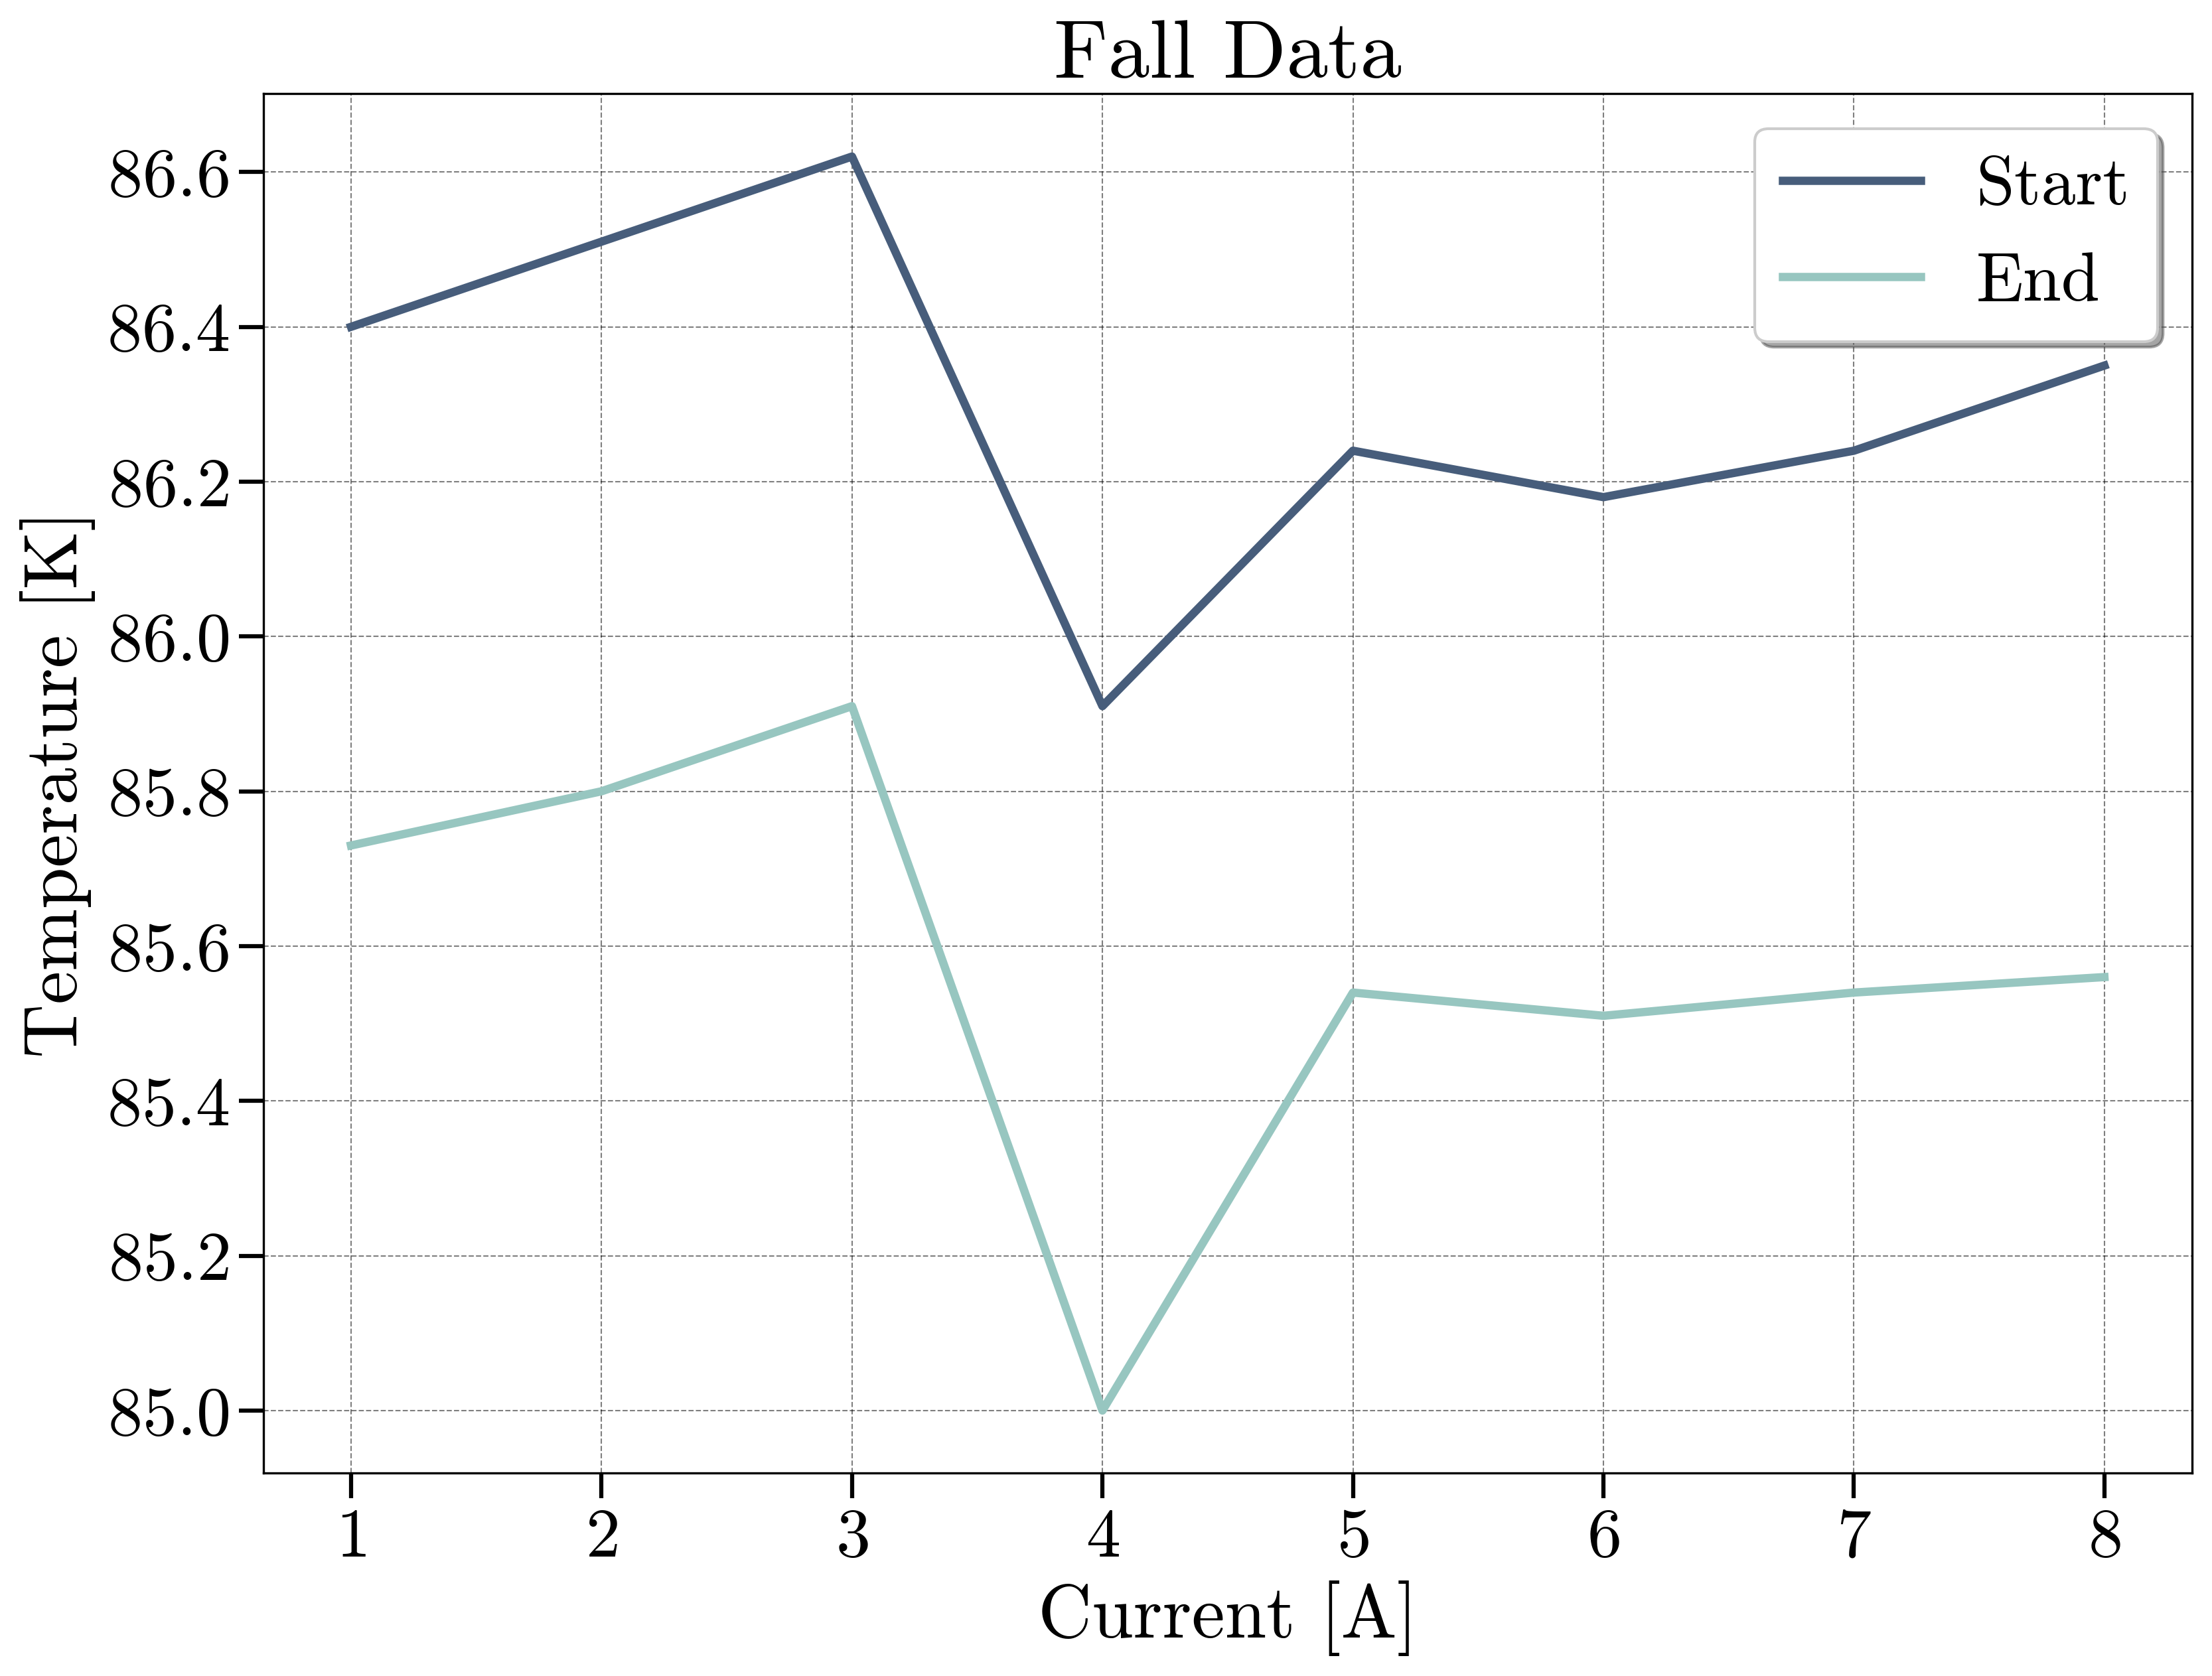
\includegraphics[width=\linewidth]{8.png}
		\caption{降温过程的转变温度与线圈电流的关系}
		\label{fig:8}
	\end{minipage}
	\hspace{0.04\linewidth}
	\begin{minipage}{0.4\linewidth}
		\centering
		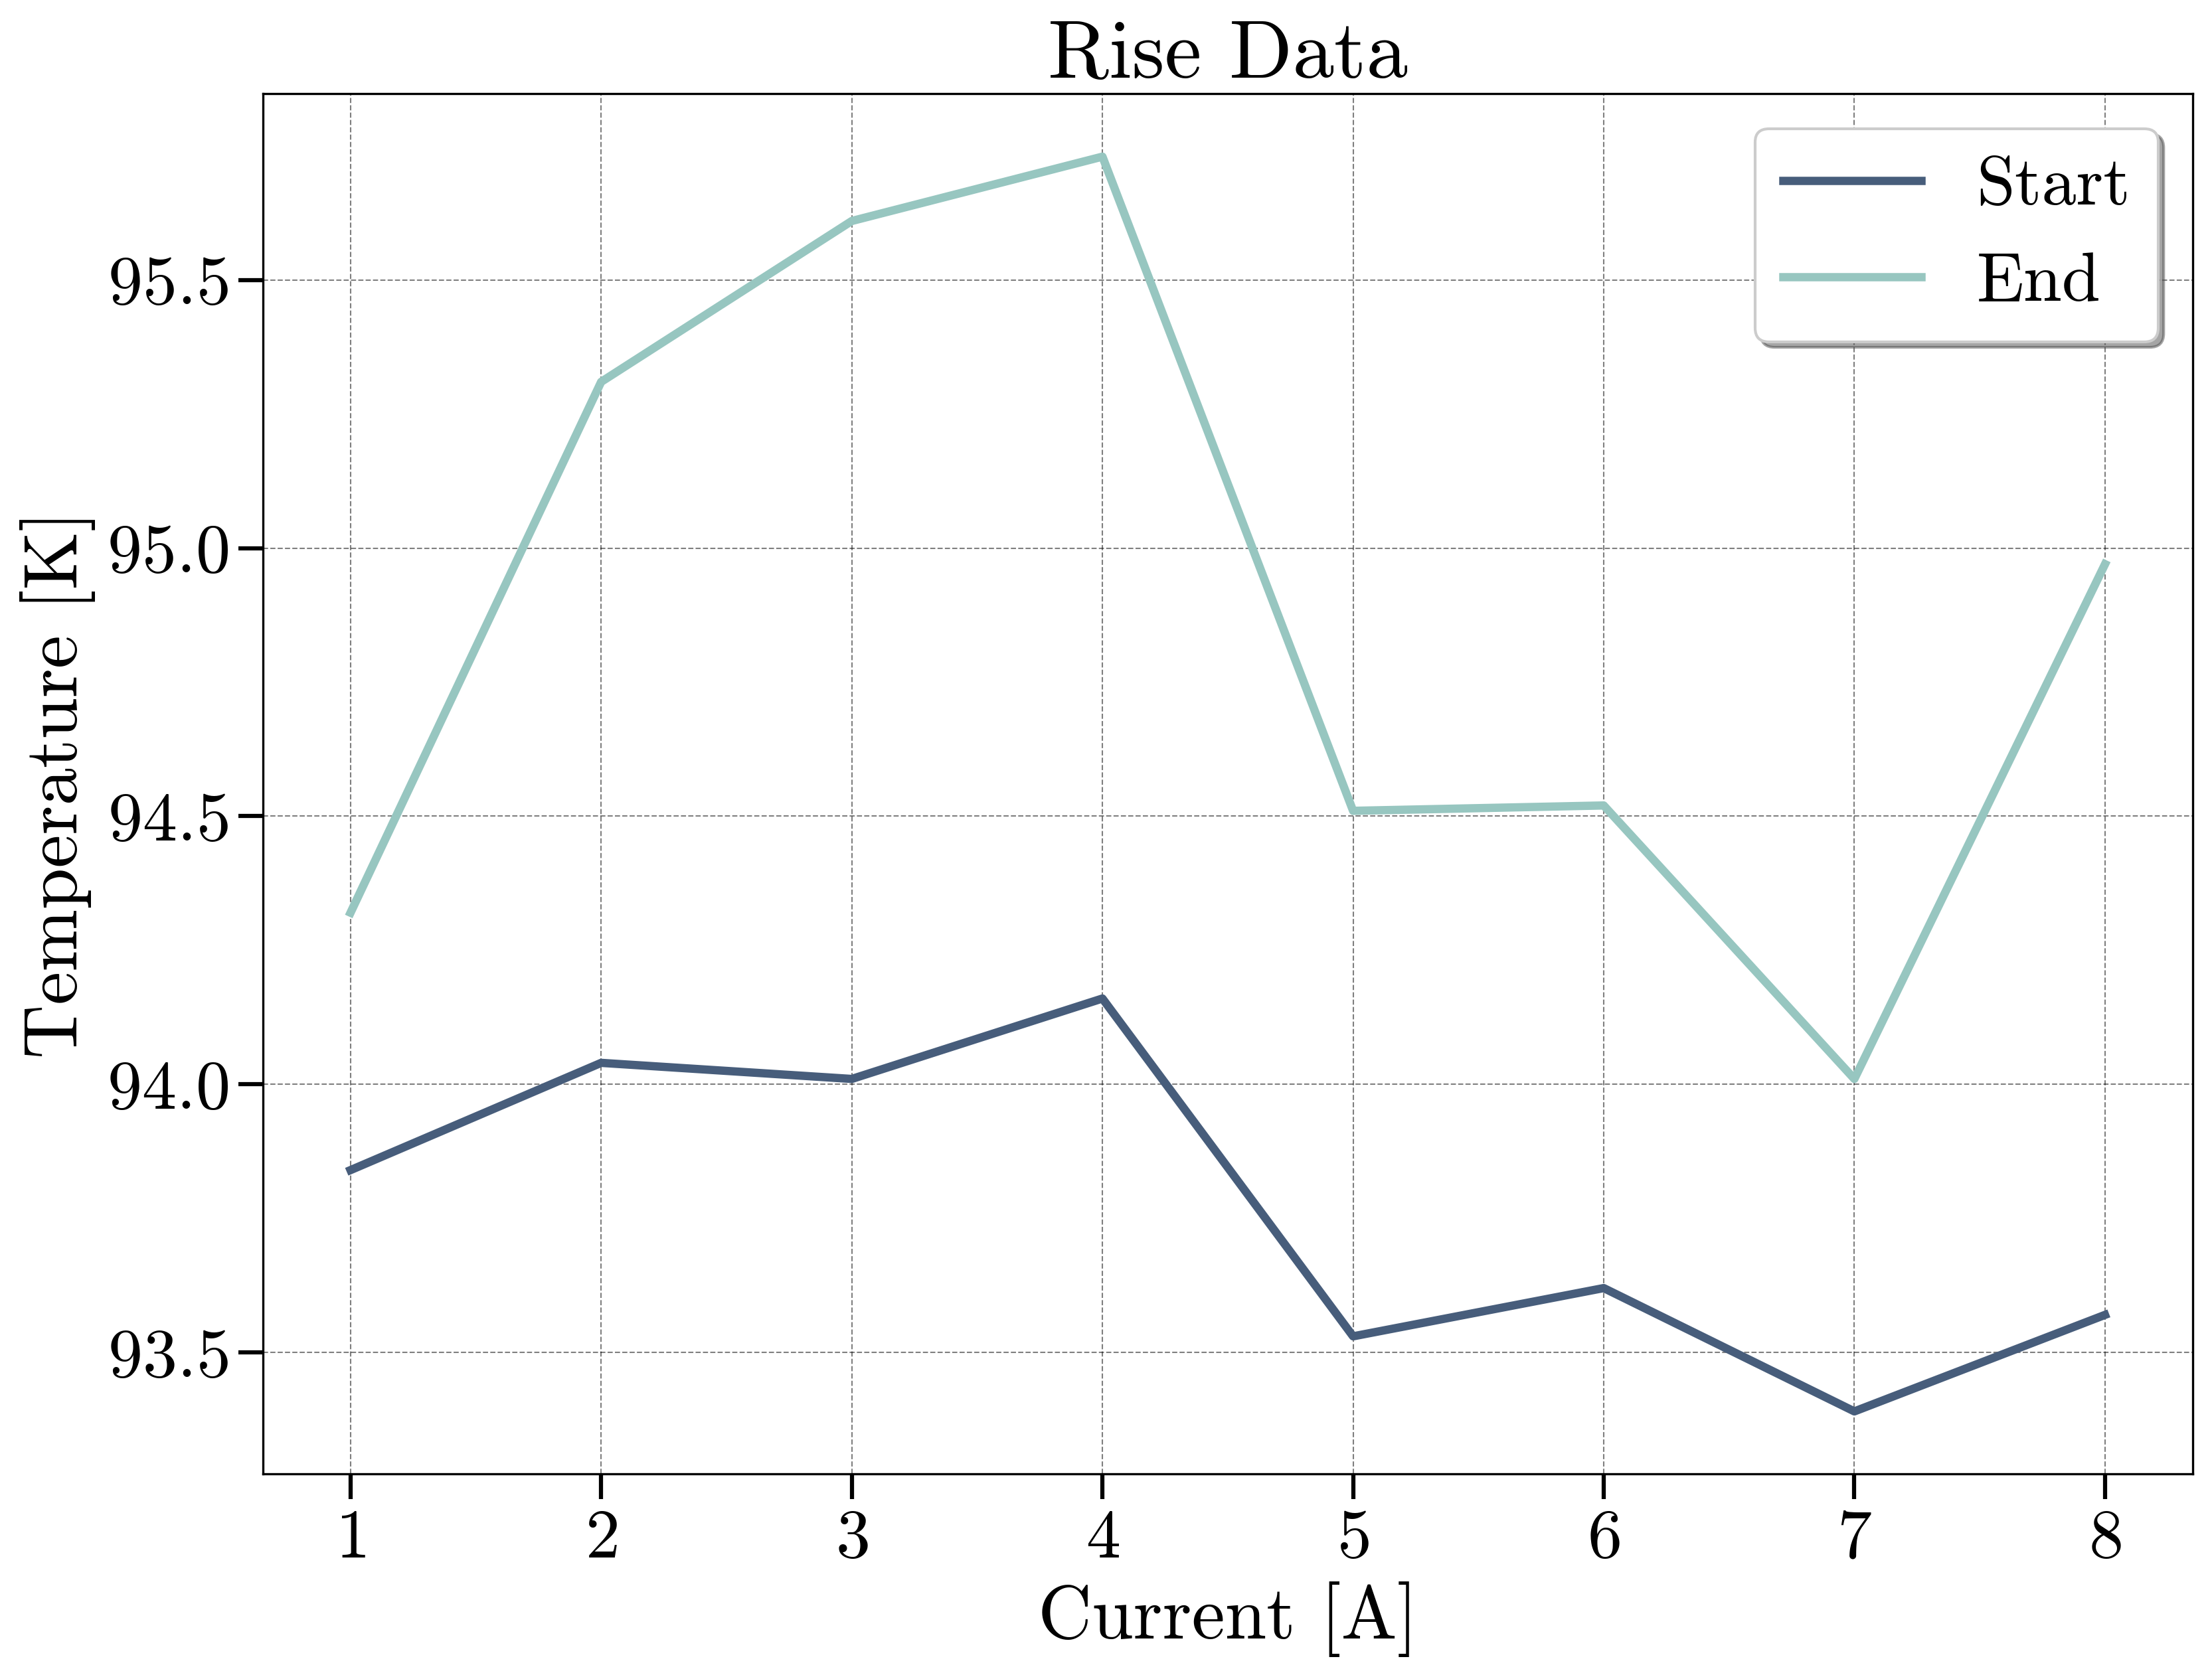
\includegraphics[width=\linewidth]{7.png}
		\caption{升温过程的转变温度与线圈电流的关系}
		\label{fig:7}
	\end{minipage}
\end{figure}


图\ref{fig:8}和\ref{fig:7}分别展示的是样品在降温和升温过程的转变温度与线圈电流的关系。

从图中可以看出,该样品的转变温度变化对外磁场并不敏感,转变温度的上下波动更多的是测量误差。
\subsubsection{理论建模}
\JMEmph{但是实际上,根据理论模型,本实验的操作会给出如下的预期实验结果:}

超导体的超导转变温度(临界温度 $T_c$)受到外加磁场的影响,外磁场的作用主要表现为两个方面:
\begin{itemize}
    \item \textbf{磁场对超导电子配对的破坏作用}:超导现象的本质是库珀对(Cooper pairs)的形成,这些配对的电子在无外磁场时通过相互吸引形成超导态。当施加外磁场时,磁场会破坏这些库珀对,因为磁场会破坏电子对的相干性。
    \item \textbf{临界磁场的存在}:每种超导材料都有一个特定的临界磁场($H_{c}$),超过这个临界磁场,超导体就会转变为正常态。外加的磁场会影响超导体的临界温度,因此,随着外磁场的增大,超导体的临界温度会降低。
\end{itemize}
\begin{figure}[{H}]
	\centering
	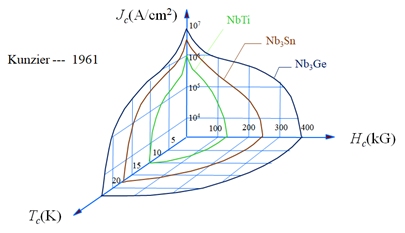
\includegraphics[width=0.6\linewidth]{9.png}
	\caption{超导临界温度、临界电流密度与临界磁场之间的关系}
	\label{}
\end{figure}

阿尔希博格-吉尔伯特模型

在低温下,超导体的临界温度 $T_c$ 与外加磁场 $H$ 之间的关系可以用经验公式来描述。对于许多超导体(如高温超导体 YBa$_2$Cu$_3$O$_{7-\delta}$),这种关系可以近似表示为:
\[
T_c(H) = T_c(0) \left(1 - \frac{H}{H_{c2}}\right)
\]
其中:
\begin{itemize}
    \item $T_c(H)$ 是在磁场 $H$ 下的超导临界温度;
    \item $T_c(0)$ 是在零磁场下的超导临界温度;
    \item $H_{c2}$ 是超导体的二级临界磁场(即磁场强度达到 $H_{c2}$ 时,超导状态完全消失)。
\end{itemize}

该公式表明,随着外磁场的增大,临界温度 $T_c$ 会线性下降,直到在临界磁场 $H_{c2}$ 处,临界温度完全为零,超导体失去超导性质。

此外,外磁场不仅影响超导临界温度,还会影响超导转变的过程。随着外磁场的增大,超导体的超导转变过程变得更加缓慢。这是因为:
\begin{itemize}
    \item \textbf{库珀对的破坏}:外磁场破坏了库珀对的形成,因此超导转变的过程变得更加平缓。
    \item \textbf{涡旋动态的引入}:在高磁场下,超导体内部会形成涡旋(vortices)。涡旋是磁场线通过超导体的区域,其中超导电流不能流动,从而增加了磁场下的能量损失,并使得超导转变变得更加缓慢。
\end{itemize}

\JMEmph{根据上述理论,当外磁场逐渐增大时,超导临界温度会下降,并且转变过程变得更加缓慢,但是根据实际的实验数据并不能得出如此结论。}

\subsection{实验进一步讨论}
\subsubsection{温度的测量}

理论上,我们预期的结果应该是,不论是升温过程还是降温过程,都有相同的转变温度;但是实际实验的测量结果显示,升温过程的转变温度为94K左右,降温过程的转变温度为86K左右,相差8K,这已经超出了简单的“测量误差”的接受范围。

\JMEmph{一个可能的原因是温度传感器的温度并未真实的反应样品的温度,而是存在一个滞后。}在我们的实验中,升温与降温采用动态法测量,温度变化速率不同,导致样品与温度计的温度响应存在差异。\JMEmph{升温时,温度计显示温度比样品实际温度高,测得转变温度偏高;降温时,温度计显示温度比样品实际温度低,测得转变温度偏低。}

一个改进的方向是,降低温度变化的速率,让被测样品与温度传感器之间达到热平衡,以此测得更准确的温度。

\subsubsection{电阻的测量}

理论上,我们应当预期在超导转变前后,样品具有相同的电阻值;但是测量结果显示,在反复测量的过程中,测量得到的电阻值存在较大的波动。

可能的原因是,我们所使用的压控电流源并不稳定,这会导致锁相放大器所测量得到的电压值也不稳定,造成较大的波动。

另一个可能的原因是,样品中可能存在温度梯度,会产生热电效应,导致额外的电压或电流,从而影响测量结果。



\subsection{总结讨论}

\begin{ubox}{实验结果}
	\quad \quad 总的来说,实验并没有得出一个合适的结果,尽管我们找到了超导转变温度带来的陡升和陡降,但是从结果来看,我们无法分析出符合理论模型的实验结果,实验数据分析部分也讨论了关于理论模型的预期结果,与我们的相差很大。
\end{ubox}
\begin{ubox}{优化方向}
	\quad \quad 我曾经在某研究所参与过一段时间的相关实验,其中某一环节需要使用到低温环境,所采用的同样是液氮降温,采用的与本实验中类似的恒温装置——一个低温杜瓦,根据当时的实验结果的数据来看,的确做到了正常的工作状态。
    \begin{figure}[H]
        \centering
        \begin{minipage}{0.3\textwidth} % 设置图片宽度
            \centering
            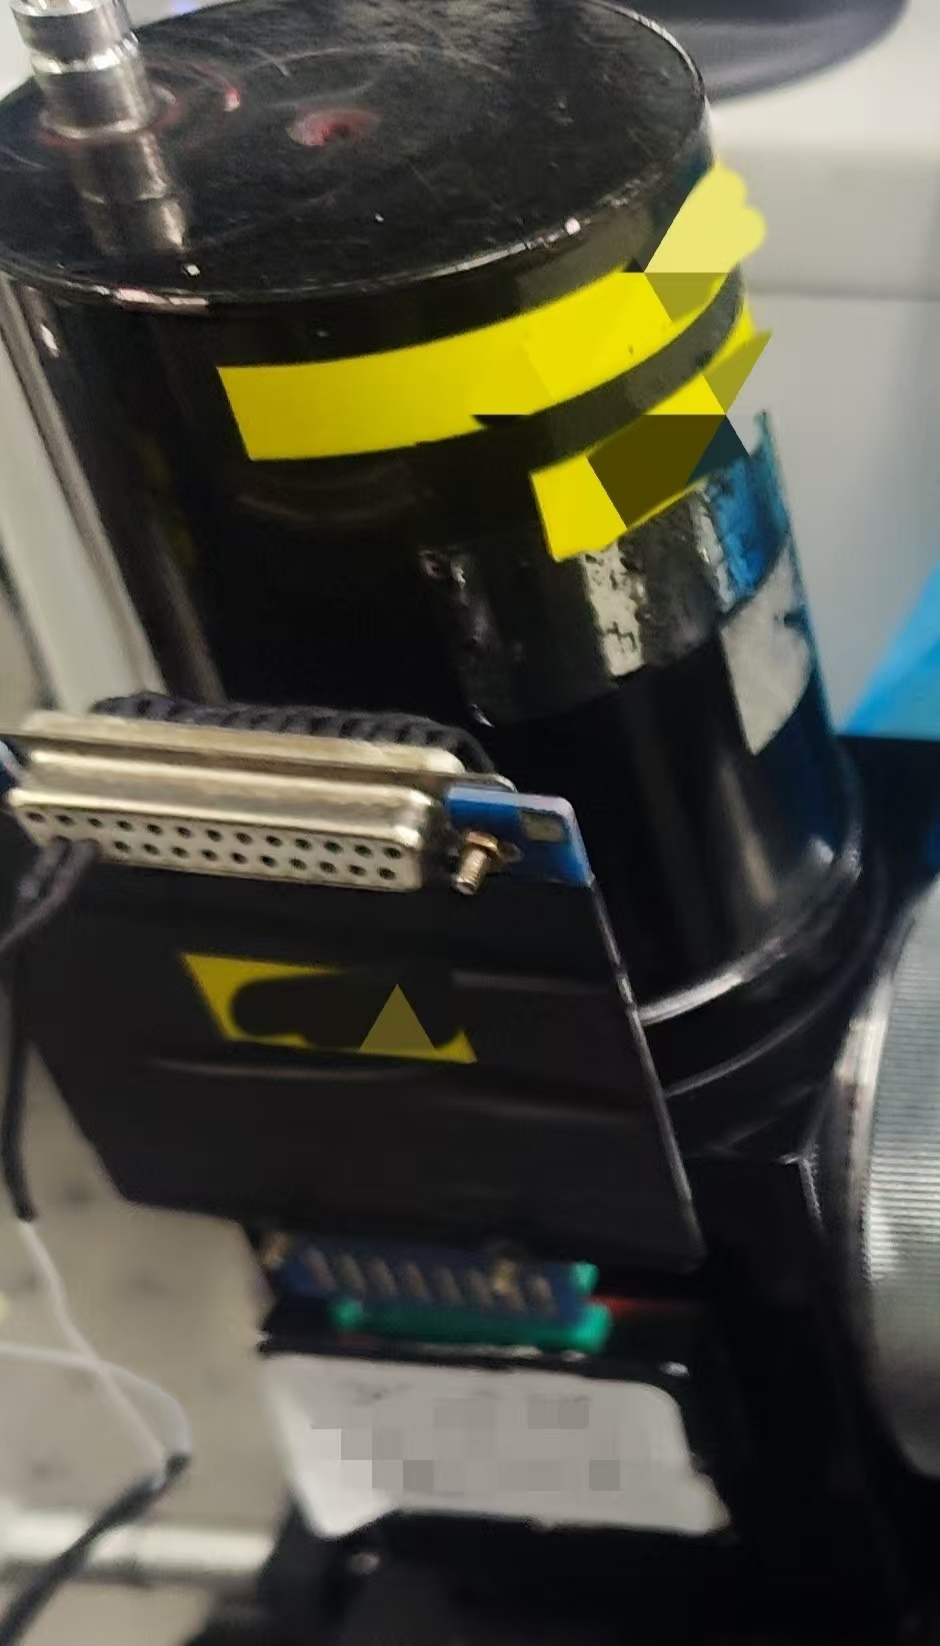
\includegraphics[width=\linewidth]{body5.jpg}
            \caption{低温杜瓦}
        \end{minipage}%
        \hfill
        \begin{minipage}{0.55\textwidth} % 设置文字的宽度
			\quad \quad 受此启发,对于实验中使用的漏热式液氮恒温器结构,我觉得一个优化方向是,提高实验装置的集成,通过设计紧凑型的低温杜瓦,能够将温控设备与样品测量系统更紧密地结合,减少热损失,提高实验的响应速度。\JMEmph{但是可能受限于样品本身的制作,以及具体仪器的尺寸问题。}
            
			\quad \quad 此外,增加集成的另一个方向是,实验仪器中,我们连接了大量的接线进行实验,比如为了分出锁相放大器的A和B,我们连接了很繁琐的电路将其分开,这些接线带来的误差也可能对于实验结果产生影响,数据存在抖动(有些抖动极大),所以对于实验电路的集成也是优化方向之一。

            \quad \quad 最后,实验的控温算法也是优化方向之一,首先功率只有三挡,并且挡位与仪器实际的升温降温的环境并不匹配,这就导致了,功率低升不上去,功率高升得太快,从而导致了,温度测量延迟等问题;由于控温采用的时PID控温,参数的设定是否符合实验仪器本身,也可能导致实际控温效果较差,导致了最后实验结果的失败。
        \end{minipage}
    \end{figure}
\end{ubox}




